%
% File: example11.tex
%
% Description: Test \label, \ref, \toclabel, and \tocref
%

\documentclass[12pt]{article}
\usepackage{edXpsl} % edX style file

\begin{document}
%%%%%%%%%%%%%%%%%%%%%%%%%%%%%%%%%%%%%%%%
\begin{edXcourse}{1.00x}{1.00x Fall 2014}[url_name=2014_Fall showanswer=always start=2014-10-06T12:00]

%%====================================== CHAPTER 0
\begin{edXchapter*}{Module 0}[start="2014-10-04"]
\toclabel{chap:intro}

%%-------------------------------------- SEQUENTIAL 0-1: Problem Set 0
\begin{edXsequential}{A problem section}[due="2014-10-22" graded=true]

\begin{edXtext}{Objective}

Measurable outcomes for this section:
\begin{enumerate}
  \item \toclabel{mo:explore} Explore the edX platform
  \item Answer an edX question \toclabel{mo:problem}
\end{enumerate}

Example unnumbered figure:
\begin{figure}
  \begin{center}
    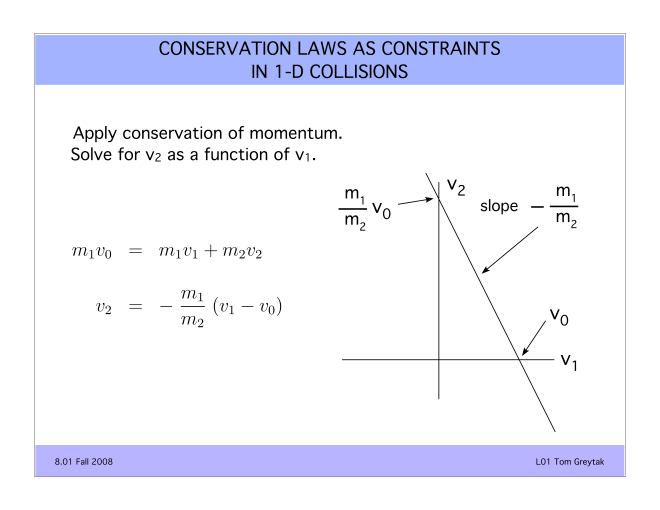
\includegraphics{example-image}
  \end{center}
\end{figure}

Example numbered figure: %note that in the example below, the line breaks are unnecessary
\begin{figure}
  \begin{center}
    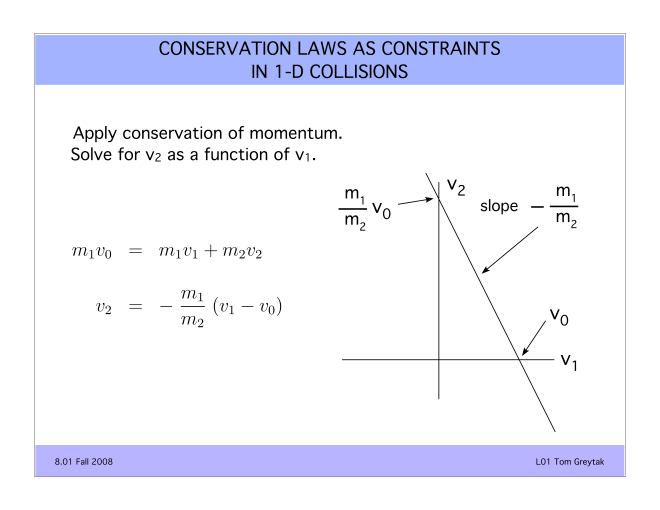
\includegraphics{example-image.png}
    \caption{Example single figure}

    \label{fig:single}

  \end{center}
\end{figure}

Example equation:
\begin{equation}
  c^2 = a^2 + b^2
  \label{eq:pythagorean}
\end{equation}

Example multifigure:
\begin{figure}
  \begin{center}
    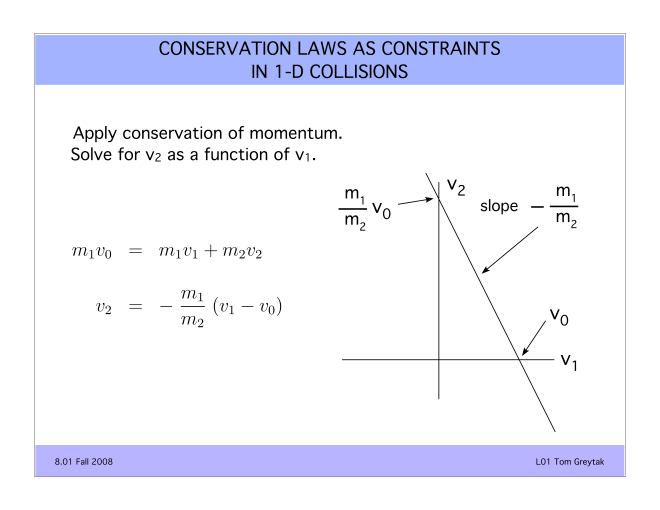
\includegraphics{example-image.png}
    \hfill
    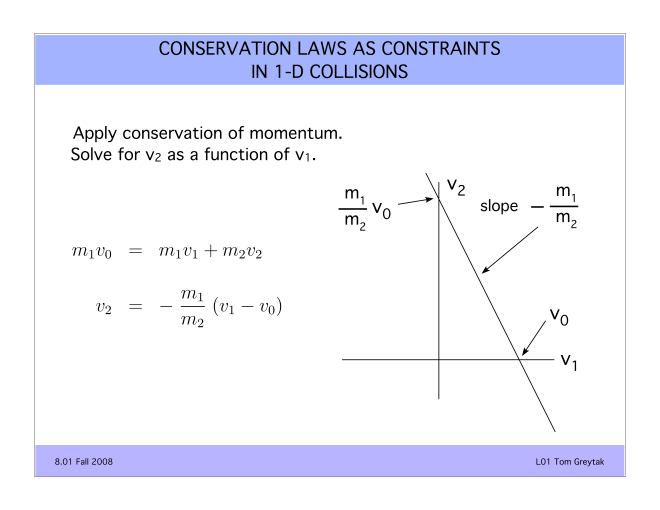
\includegraphics{example-image.png}
    \caption{Example multifigure}
    \label{fig:multi}
  \end{center}
\end{figure}

\end{edXtext}

\begin{edXproblem}{Example problem}{url_name="p0"}
\tocref{mo:explore} \tocref{mo:problem}

First example question for the first learning objective (a.k.a measurable outcome).

\end{edXproblem}

\end{edXsequential}

%%--------------------------------------
\end{edXchapter*}

%%====================================== CHAPTER 1
\begin{edXchapter}{Module 1}[start="2014-10-06"]

% Hidden Learning Objectives, should only appear in ToC
\begin{enumerate}
  \item Complete \toclabel{mo:hidden} the course
\end{enumerate}

%%-------------------------------------- SEQUENTIAL 1-1: Lecture 1
\begin{edXsequential}{A lecture section}
\label{sec:lecture1}

\begin{edXtext}{Example text}[url_name="text-L1"]
\tocref{mo:explore} \tocref{mo:undefined}

In Section \ref{chap:intro} we saw example figure references.  Here are some equations.

Example equation:
\begin{equation}
  \frac{d}{dx} e^x = e^x
  \label{eq:deriv}
\end{equation}

Example equation array:
\begin{eqnarray}
  z & = x \times y \label{eq:com1}\\
  z & = y \times x \label{eq:com2}
\end{eqnarray}

The fact that for scalars Equation \ref{eq:com1} is equal to Equation \ref{eq:com2} is known as the commutative property.

The label for this reference \ref{eq:unused} has not been defined.

\end{edXtext}

\end{edXsequential}

%%-------------------------------------- SEQUENTIAL 1-2: Lecture 2
\begin{edXsequential}{Another lecture section}

% EVH Not sure if this appears anywhere in the course
\begin{enumerate}
  \item Another hidden item \label{it:random}
\end{enumerate}

\begin{edXvertical}{A vertical grouping}
\label{subsec:group1}

\begin{edXtext}{More references}

In this sequential, we have a vertical element with introductory text and a Figure \ref{fig:examplefig}.
\begin{figure}
  \begin{center}
    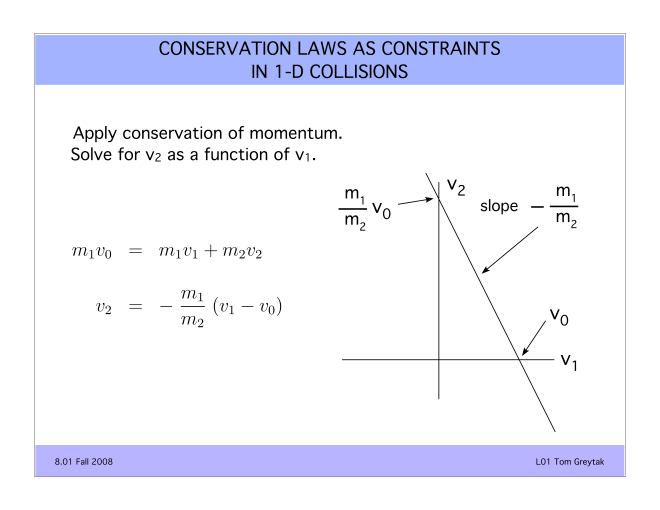
\includegraphics{example-image.png}
    \caption{Example single figure}
    \label{fig:examplefig}
  \end{center}
\end{figure}

\end{edXtext}

\begin{edXproblem}{Example Problem 1}{url_name="p1"}

Followed by a problem with an Equation \ref{eq:sum}.
\begin{equation}
  \boxed{A = B + C}
  \label{eq:sum}
\end{equation}

\end{edXproblem}

\end{edXvertical}

\end{edXsequential}

%%--------------------------------------
\end{edXchapter}

%%======================================
\end{edXcourse}

\end{document}
